\documentclass{beamer}
\usepackage{amsfonts}
\usepackage{amsmath}
\usepackage{times}
\usepackage{mathrsfs}
\usepackage{extarrows}
\usepackage{bbm} 
\setbeamercolor{footcolor}{fg=blue!100} % 设置字体和背景颜色
\setbeamertemplate{headline}{%
  \leavevmode%
  \hbox{%
    \hskip228pt
    \begin{beamercolorbox}[wd=.126\paperwidth,ht=2.25ex,dp=1ex,right]{footcolor}%      
       \textcolor[rgb]{0,0.168,0.376}{Slide \insertframenumber{} }
    \end{beamercolorbox}}%
  \vskip-19pt%
}

\setbeamertemplate{frametitle}
{
\vspace{30pt}\textcolor[rgb]{0,0.168,0.376}{\insertframetitle}
}

 
\pgfdeclareimage[height=0.61cm]{university-logo}{logo.png}  
\logo{\pgfuseimage{university-logo}{\vspace{244pt}}} 
\title{\textcolor[rgb]{0,0.168,0.376}{VV286 RC6}}
\author{JIANG Yicheng}
\begin{document}

\begin{frame}
\titlepage
\end{frame}




\begin{frame}
\frametitle{The (Unilateral) Lapalace Transform}
Let $f:[0,\infty)\rightarrow\mathbb{R}$ be a continuous function such that
$$\sup_{t\in[0,\infty)}e^{-\beta t}|f(t)|<\infty\hspace{3mm}\text{for some }\beta\geqslant0$$
Then the function $F:(\beta,\infty)\rightarrow\mathbb{R}$,
$$F(p)=(\mathscr{L} f)(p)=\int_0^{\infty}e^{-pt}f(t)dt$$
is called the Lapalace transform of $f$.


\end{frame}


\begin{frame}
\begin{figure}[h]
    \centering
    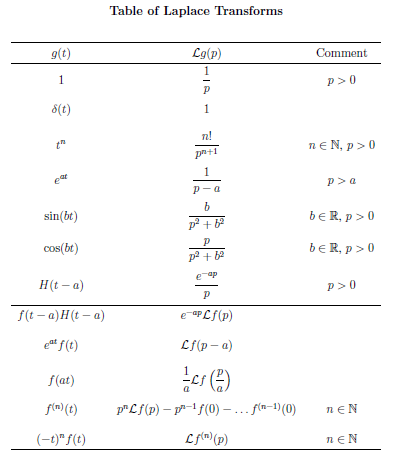
\includegraphics[height=8.2cm]{lapalace.png}
\end{figure}
\end{frame}

\begin{frame}
\begin{block}{Heaviside function}
$$H:\mathbb{R}\mapsto\mathbb{R},\hspace{5mm}H(t)=\left\{
\begin{aligned}
&1,t>0\\
&0,t\leqslant0\\
\end{aligned}
\right.$$
\end{block}

\begin{block}{Delta function (not a function at all)}
\begin{enumerate}
\item For $t\neq0$,
$$\delta(t)=0$$
\item $0\in I\subset\mathbb{R}$
$$\int_I\delta(t)f(t)dt=f(0)$$
\end{enumerate}
\end{block}
\end{frame}

\begin{frame}
\frametitle{Inverting the Lapalace Transform}
\begin{block}{The Bromwich Integral}
Let $\Omega \subset \mathbb{C}$ be an open set, $\beta\in \mathbb{R}$ and $F :\Omega \rightarrow\mathbb{C}$ analytic for all $z \in \mathbb{C}$ with $\text{Re} z \geqslant\beta$. Then the Bromwich integral of $F$ is
$$(\mathscr{M}F)(t) =\dfrac{1}{2\pi i}\int_{\mathcal{C}^*}e^{pt}F(p) dp=\dfrac{1}{2\pi i}\int_{\beta-i\infty}^{\beta+i\infty}e^{pt}F(p) dp$$
\begin{enumerate}
\item For $t > 0$, the Bromwich integral $\mathscr{M}F(t)$ is usually calculated by closing the contour on the left and applying the residue theorem.
\item For $t < 0$ we close the contour on the right.
\end{enumerate}
(To use Jordan's Lemma)
\end{block}
\end{frame}

\begin{frame}

\begin{block}{Convolution}
$$(f * g)(t) :=\int^t_0f (t-s)g(s) ds$$
$$(\mathscr{L})(f*g)=(\mathscr{L}f)\cdot(\mathscr{L} g)$$
\end{block}
\end{frame}

\begin{frame}
\begin{block}{Solving an ODE with the Laplace Transform}
To deal with discontinuous inhomogeneities and even inhomogeneities that are not functions at all.
$$ay''+by'+cy=f(x),\,\,\,y(0)=y_0,\,\,\,y'(0)=y_1$$
\end{block}
\begin{block}{1.}
Apply the Laplace transform to both sides of the ODE/IVP;
\begin{align*}
(\mathscr{L}f')(p)&=\int_0^{\infty}e^{-pt}f'(t)dt=\int_0^{\infty}pe^{-pt}f(t)dt-f(0)\\
&=p\cdot(\mathscr{L}f)(p)-f(0)\\
(\mathscr{L}f'')(p)&=p^2(\mathscr{L}f)(p)-p\cdot f(0)-f'(0)
\end{align*}
$$(ap^2+bp+c)Y-(ap+b)y_0-ay_1=(\mathscr{L}f)(p)$$
\end{block}
\end{frame}

\begin{frame}
\begin{block}{2.}
$$Y=(\mathscr{L}f)(p)\cdot\dfrac{1}{ap^2+bp+c}+\dfrac{ay_0p+by_0+ay_1}{ap^2+bp+c}$$
Find $g(x)$ such that $(\mathscr{L}g)(p)=\dfrac{1}{ap^2+bp+c}$

The function $g$ is called a Green's function for the differential
equation.
\end{block}
\begin{block}{3. }
Use transform table and apply convolution to find inverse Laplace transform.
\end{block}
\end{frame}

\begin{frame}
\begin{block}{Example}
$$y''+y=\left\{
\begin{aligned}
&\cos t,0\leqslant t\leqslant\pi/2\\
&0,\pi/2\leqslant t<\infty\\
\end{aligned}
\right.=\cos t\cdot H(\dfrac{\pi}{2}-t),y(0)=3,y'(0)=-1$$
\end{block}
\end{frame}

\begin{frame}
\begin{block}{Solution}
Set $Y(p)=(\mathcal{L}y)(p)$, then
$$(\mathcal{L}y')(p)=p\cdot(\mathcal{L}y)(p)-y(0)=pY(p)-3 $$
$$(\mathcal{L}y'')(p)=p\cdot(\mathcal{L}y')(p)-y'(0)=p^2Y(p)-3p+1 $$

So apply Laplace transform to the equation and we get
\begin{align*}
&(p^2+1)Y(p)=\mathcal{L}(\cos t\cdot H(\dfrac{\pi}{2}-t))+3p-1\\
\Rightarrow& Y(p)=\dfrac{1}{p^2+1}\cdot \mathcal{L}(\cos t\cdot H(\dfrac{\pi}{2}-t))+3\dfrac{p}{p^2+1}-\dfrac{1}{p^2+1}\\
\Rightarrow& Y(p)=\mathcal{L}(\sin t)\cdot\mathcal{L}(\cos t\cdot H(\dfrac{\pi}{2}-t))+3\mathcal{L}(\cos t)-\mathcal{L}(\sin t)
\end{align*}
\end{block}
\end{frame}


\begin{frame}
\begin{block}{}
For $t\geqslant\dfrac{\pi}{2}$
\begin{align*}
&(\sin t)*(\cos t\cdot H(\dfrac{\pi}{2}-t))\\
=&\int_0^t (\sin (t-s)(\cos s\cdot H(\dfrac{\pi}{2}-s))ds \\
=&\dfrac{1}{2}\int_0^{\frac{\pi}{2}} \sin t+\sin(t-2s) ds\\
=&\dfrac{1}{2} (s\sin t\big|_0^{\frac{\pi}{2}}+\dfrac{1}{2}\cos(t-2s)\big|_0^{\frac{\pi}{2}})\\
=&\dfrac{\pi}{4}\sin t-\dfrac{1}{2}\cos t
\end{align*}
\end{block}
\end{frame}

\begin{frame}
\begin{block}{}
For $0\leqslant t<\dfrac{\pi}{2}$
\begin{align*}
&(\sin t)*(\cos t\cdot H(\dfrac{\pi}{2}-t))\\
=&\int_0^t (\sin (t-s)(\cos s\cdot H(\dfrac{\pi}{2}-s))ds =\dfrac{1}{2}\int_0^{t} \sin t+\sin(t-2s) ds\\
=&\dfrac{1}{2} (s\sin t\big|_0^{t}+\dfrac{1}{2}\cos(t-2s)\big|_0^{t})\\
=&\dfrac{t}{2}\sin t
\end{align*}
\end{block}
\end{frame}

\begin{frame}
\begin{block}{}
So 
$$y(t)=\left\{
\begin{aligned}
&(\dfrac{\pi}{4}-1)\sin t+\dfrac{5}{2}\cos t,t\geqslant \dfrac{\pi}{2}\\
&(\dfrac{t}{2}-1)\sin t+3\cos t,0\leqslant t<\dfrac{\pi}{2}\\
\end{aligned}
\right.
$$
\end{block}
\end{frame}

\begin{frame}
\frametitle{The Fourier Transform}
\begin{block}{}
Let $f:\mathbb{R}\rightarrow\mathbb{C}$, if $f$ is absolutely integrable, i.e.
$$\int_{-\infty}^{\infty}|f(x)|dx<\infty$$ 
Then
$$\widehat{f}(\xi)=\dfrac{1}{\sqrt{2\pi}}\int_{-\infty}^{\infty}f(x)e^{-i\xi x}dx$$
exists for all $\xi\in\mathbb{R}$. $\widehat{f}(\xi)$ is called the Fourier Transform of $f$.

\end{block}
\end{frame}


\begin{frame}
\begin{block}{Properties}
\begin{enumerate}
\item $$\widehat{(f')}(\xi)=i\xi\cdot\widehat{f}(\xi)$$
\item $$\dfrac{d}{d\xi}\widehat{f}(\xi)=\widehat{(-ix)f}(\xi)$$
\item 
$$\widehat{(f(ax))}(\xi)=\dfrac{1}{|a|}\widehat{f(x)}(\dfrac{\xi}{a})$$
\item
$$\widehat{(e^{iat}f)}(\xi)=\widehat{f}(\xi-a)$$ 
\end{enumerate}

\end{block}
\end{frame}

\begin{frame}
\begin{block}{Decay}
Let $\Omega \subset \mathbb{R}$ be bounded and $f : \mathbb{R}\setminus \Omega
\rightarrow \mathbb{C}$.
\begin{enumerate}

\item  If $ f (x) = O(x^{-n})$ as $|x|\rightarrow\infty$  for some $n > 0$, then $f$ is said to have polynomial decay at infinity.
\item  If $ f (x) = O(x^{-n})$ as $|x|\rightarrow\infty$ for all $n > 0$, then $f$ is said to have faster-than-polynomial decay at infinity.
\item  If $ f (x) = O(e^{-b|x|})$ as $|x|\rightarrow\infty$ for some $b > 0$, then $f$ is said to have exponential decay at infinity.
\end{enumerate}
\end{block}
\end{frame}


\begin{frame}
\begin{block}{Decay Behavior of Fourier Transform}
\begin{enumerate}
\item If $f \in C^{\infty}(\mathbb{R})$ and all derivatives of $f$ are absolutely integrable, then $\widehat{f}$ has faster-than-polynomial decay at infinity.
\item If $f$ is analytic on $S_a=\lbrace z \in \mathbb{C}: |\text{Im} z| < a\rbrace$ for some $a>0$ and there exists a constant $A>0$ such that
$$f(z)=f(x+iy)\leqslant\dfrac{A}{1+x^2}$$
for all $z=x+iy\in S_a$, (denote the set of all such kind of $f$ as $\mathscr{F}_a$), then for any $0 \leqslant b < a$ there exists a constant $B > 0$ such that 
$$|\widehat{f}(\xi)|\leqslant Be^{-b|\xi|}$$
 for all $ \xi\in\mathbb{R} $. ($\widehat{f}$ has exponential decay at infinity.)
\end{enumerate}

\end{block}
\end{frame}


\begin{frame}
\frametitle{Fourier Inversion Theorem}
$\forall f\in\mathscr{F}=\bigcup\limits_{\forall a\in\mathbb{R}^+}\mathscr{F}_a$, $\widehat{f}$ exists and
$$f(x)=\dfrac{1}{\sqrt{2\pi}}\int_{-\infty}^{\infty}\widehat{f}(\xi)e^{i\xi x}d\xi$$
for all $x\in\mathbb{R}$

\end{frame}

\begin{frame}
\begin{block}{The Complex Fourier Transform}
For $f : \mathbb{C}\rightarrow \mathbb{C}$ define the Fourier transform of $f$ at $\xi + i\eta\in \mathbb{C}$ by 
$$\widehat{f}(\xi+i\eta)=\dfrac{1}{\sqrt{2\pi}}\int_{-\infty}^{\infty}f(x)e^{-i(\xi+i\eta) x}dx$$
\end{block}
\begin{block}{}
Let $f :\mathbb{R}\rightarrow \mathbb{R}$ satisfies $f (x) = O(e^{-b|x|})$ as $|x| \rightarrow \infty$ for some $b > 0$. Then $\widehat{f}$ exists and is analytic in the strip $S_b = \lbrace z \in\mathbb{C}:|\text{Im} z| < b\rbrace$.
\end{block}

\end{frame}

\begin{frame}
\begin{block}{Fourier Inversion Formula}
$f(x)$ is piecewise continuous, absolutely integrable, and continuously differentiable on each small interval $(a_k,a_{k+1})$ 
$$\dfrac{f(x^+)+f(x^-)}{2}=\dfrac{1}{\sqrt{2\pi}}\lim\limits_{R\rightarrow\infty}\int_{-R}^R\widehat{f}(\xi)e^{ix\xi}d\xi$$
$$f(x^+)=\lim\limits_{y\searrow x}f(y),\hspace{3mm}f(x^-)=\lim\limits_{y\nearrow x}f(y)$$
\end{block}
\end{frame}
\begin{frame}
\begin{block}{Lapalace Transform}
$$(\mathscr{L} f)(p)=\int_0^{\infty}e^{-pt}f(t)dt$$
$$(\mathscr{M}F)(t) =\dfrac{1}{2\pi i}\int_{\beta-i\infty}^{\beta+i\infty}e^{pt}(\mathscr{L} f)(p) dp$$
\end{block}
\begin{block}{Fourier Transform}
$$\widehat{f}(\xi)=\dfrac{1}{\sqrt{2\pi}}\int_{-\infty}^{\infty}f(x)e^{-i\xi x}dx$$
$$f(x)=\dfrac{1}{\sqrt{2\pi}}\int_{-\infty}^{\infty}\widehat{f}(\xi)e^{i\xi x}d\xi$$
\end{block}
\end{frame}

\begin{frame}
\frametitle{Series Methods for Second-Order Equations}
Set $x(t)=\sum\limits_{k=0}^{\infty}a_kt^k$, then
$$x'(t)=\sum\limits_{k=1}^{\infty}ka_kt^{k-1}=\sum\limits_{k=0}^{\infty}(k+1)a_{k+1}t^{k}$$
$$x''(t)=\sum\limits_{k=2}^{\infty}k(k-1)a_kt^{k-2}=\sum\limits_{k=0}^{\infty}(k+2)(k+1)a_{k+2}t^{k}$$
Insert to find relation among coefficients $a_k,a_{k+1},a_{k+2}$. If we can find two independent solutions (usually no $t$ before $x''$, the easiest case), then we have done; else

\end{frame}
\begin{frame}
Set $x(t)=t^r\sum\limits_{k=0}^{\infty}a_kt^k$, then
$$x'(t)=\sum\limits_{k=0}^{\infty}(k+r)a_kt^{k+r-1}$$
$$x''(t)=\sum\limits_{k=0}^{\infty}(k+r)(k+r-1)a_kt^{k+r-2}$$
Insert to solve $r$.
\end{frame}
\begin{frame}
\begin{enumerate}
\item Two distinct real roots $r_1$ and $r_2$, $r_1-r_2\notin\mathbb{Z}$
$$x_1(t)=t^{r_1}\sum\limits_{n=0}^{\infty}a_nt^n,\hspace{3mm}x_2(t)=t^{r_2}\sum\limits_{n=0}^{\infty}b_nt^n$$
\item Two distinct real roots $r_1$ and $r_2$, $r_1-r_2\in\mathbb{Z}$
\begin{align*}
&x_2(t)\\
=&\dfrac{\partial}{\partial r}\Big(t^r\sum\limits_{n=0}^{\infty}a_n(r)t^n\Big)\Bigg|_{r=r_2}=t^{r}\ln t\sum\limits_{n=0}^{\infty}a_n(r)t^n+t^{r}\sum\limits_{n=0}^{\infty}a'_n(r)t^n\Bigg|_{r=r_2}\\
=&c\cdot x_1(t)\ln t+t^{r_2}\sum\limits_{n=0}^{\infty}a'_n(r_2)t^n
\end{align*}
Especially $c=1$ for $r_1=r_2$.
\end{enumerate}
\end{frame}
\begin{frame}
\begin{block}{3. Complex root}
$$x_1(t)=\text{Re}\Big(t^{r_1}\sum\limits_{n=0}^{\infty}a_nt^n\Big),\hspace{3mm}x_2(t)=\text{Im}\Big(t^{r_2}\sum\limits_{n=0}^{\infty}b_nt^n\Big)$$

\end{block}
\end{frame}

\end{document}
